%===============================================================================
% Name   : R noweb template
% Author : Sarah Modesto Sanches 
% Date   : 12/11/2021 10:50:10
%===============================================================================

\documentclass[12pt]{article}\usepackage[]{graphicx}\usepackage[]{color}
% maxwidth is the original width if it is less than linewidth
% otherwise use linewidth (to make sure the graphics do not exceed the margin)
\makeatletter
\def\maxwidth{ %
  \ifdim\Gin@nat@width>\linewidth
    \linewidth
  \else
    \Gin@nat@width
  \fi
}
\makeatother

\definecolor{fgcolor}{rgb}{0.345, 0.345, 0.345}
\newcommand{\hlnum}[1]{\textcolor[rgb]{0.686,0.059,0.569}{#1}}%
\newcommand{\hlstr}[1]{\textcolor[rgb]{0.192,0.494,0.8}{#1}}%
\newcommand{\hlcom}[1]{\textcolor[rgb]{0.678,0.584,0.686}{\textit{#1}}}%
\newcommand{\hlopt}[1]{\textcolor[rgb]{0,0,0}{#1}}%
\newcommand{\hlstd}[1]{\textcolor[rgb]{0.345,0.345,0.345}{#1}}%
\newcommand{\hlkwa}[1]{\textcolor[rgb]{0.161,0.373,0.58}{\textbf{#1}}}%
\newcommand{\hlkwb}[1]{\textcolor[rgb]{0.69,0.353,0.396}{#1}}%
\newcommand{\hlkwc}[1]{\textcolor[rgb]{0.333,0.667,0.333}{#1}}%
\newcommand{\hlkwd}[1]{\textcolor[rgb]{0.737,0.353,0.396}{\textbf{#1}}}%
\let\hlipl\hlkwb

\usepackage{framed}
\makeatletter
\newenvironment{kframe}{%
 \def\at@end@of@kframe{}%
 \ifinner\ifhmode%
  \def\at@end@of@kframe{\end{minipage}}%
  \begin{minipage}{\columnwidth}%
 \fi\fi%
 \def\FrameCommand##1{\hskip\@totalleftmargin \hskip-\fboxsep
 \colorbox{shadecolor}{##1}\hskip-\fboxsep
     % There is no \\@totalrightmargin, so:
     \hskip-\linewidth \hskip-\@totalleftmargin \hskip\columnwidth}%
 \MakeFramed {\advance\hsize-\width
   \@totalleftmargin\z@ \linewidth\hsize
   \@setminipage}}%
 {\par\unskip\endMakeFramed%
 \at@end@of@kframe}
\makeatother

\definecolor{shadecolor}{rgb}{.97, .97, .97}
\definecolor{messagecolor}{rgb}{0, 0, 0}
\definecolor{warningcolor}{rgb}{1, 0, 1}
\definecolor{errorcolor}{rgb}{1, 0, 0}
\newenvironment{knitrout}{}{} % an empty environment to be redefined in TeX

\usepackage{alltt}
\usepackage[sc]{mathpazo}
\usepackage[T1]{fontenc}
\usepackage[left=3cm, right=2cm, top=3cm, bottom=2cm]{geometry}
\usepackage[utf8]{inputenc}
\usepackage{caption}
\usepackage[portuguese]{babel}
\usepackage{booktabs}
\geometry{verbose,
 tmargin=2.5cm,
 bmargin=2.5cm,
 lmargin=2.5cm,
 rmargin=2.5cm}
\setcounter{secnumdepth}{2}
\setcounter{tocdepth}{2}
\usepackage{url}
\usepackage[unicode=true,
 pdfusetitle,
 bookmarks=true,
 bookmarksnumbered=true,
 bookmarksopen=true,
 bookmarksopenlevel=2,
 breaklinks=false,
 pdfborder={0 0 1},
 backref=false,
 colorlinks=false]{hyperref}
\hypersetup{
 pdfstartview={XYZ null null 1}}
\usepackage{breakurl}
\IfFileExists{upquote.sty}{\usepackage{upquote}}{}
\begin{document}
\begin{center}
    
\includegraphics[scale=0.2]{uesct.jpg}
    
    \textbf{Universidade Estadual de Santa Cruz}
    
    \textbf{Departamento de Ciências Exatas e Tecnológicas - DCET}

    \textbf{Curso: Engenharia Elétrica}
    
    \textbf{Discente:José Claúdio faria }
  
    \textbf{Docente: Sarah Modesto Sanches(202012319) e Kevin Moura(201811019).}
     \vspace{2cm}
     
    \Large\textbf{Análise Exploratória de dados: CET173 - Probabilidade e Estatistica}
    
    \large\textbf{Matriculas: 202012319 201811019 201811019}
    
    \large\textbf{Os dados foram simulados computacionalmente e tem finalidades apenas acadêmicas e didáticas para fins de avaliação}
   
\vfill  
    \begin{center}
        \today
        ILHÉUS-BA
    \end{center}
\end{center} 

\newpage





\section{AED: Apresentações tabulares e gráficas (2.0)}
\subsection{(1.0) Diagrama de caixa (boxplot) para Y1 e Y2:} 
       \textbf{1.1.1 (0.5) Antes e após a eliminação de possíveis outliers - sem distinção de sexo:}

\begin{figure}[!h]
\label{figura:boxplot}
\begin{knitrout}
\definecolor{shadecolor}{rgb}{0.969, 0.969, 0.969}\color{fgcolor}

{\centering 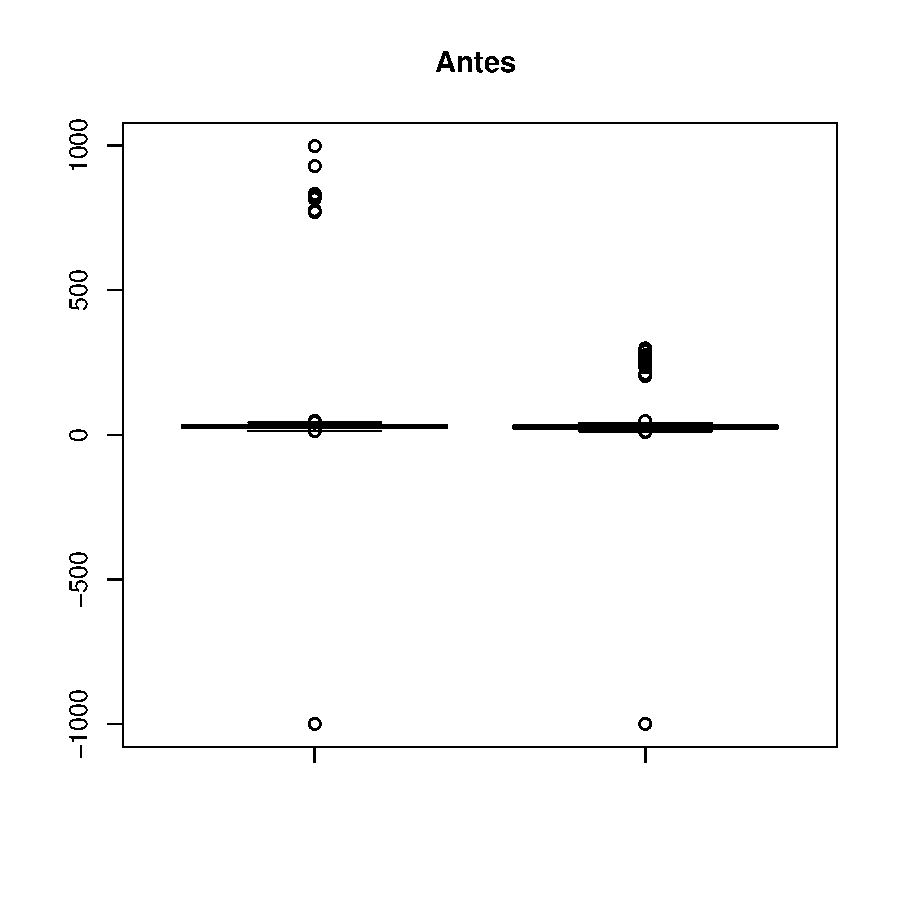
\includegraphics[width=.4\linewidth]{figure/minimal-boxplot-antes-1} 
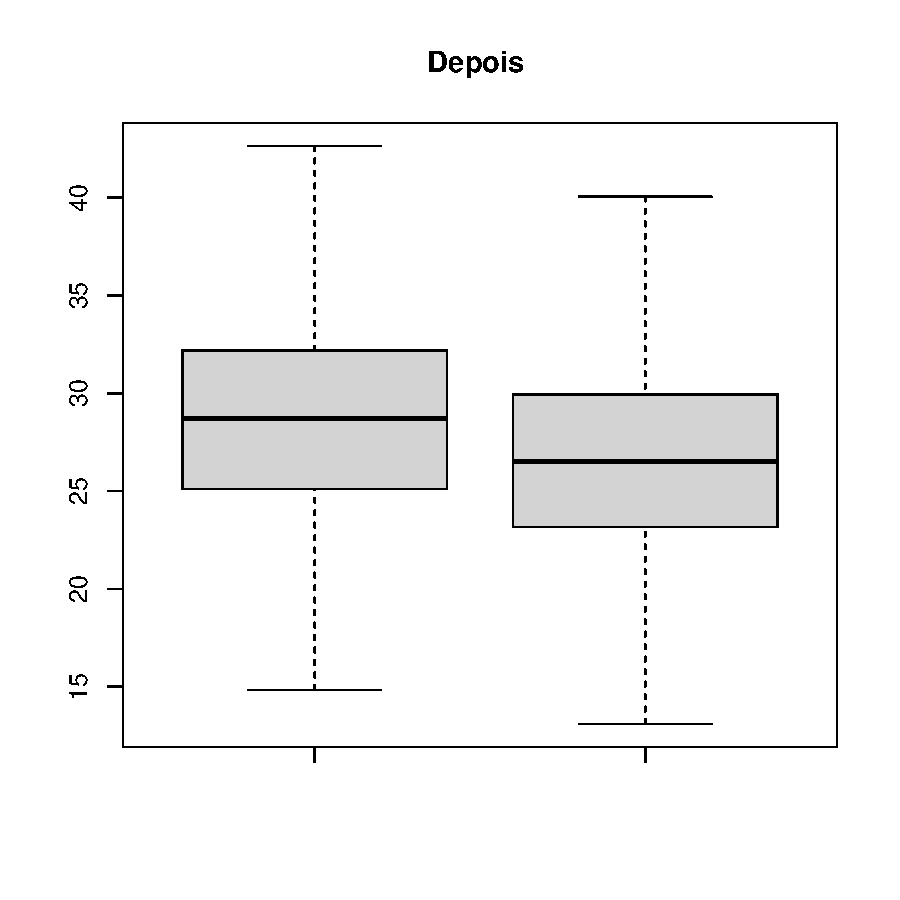
\includegraphics[width=.4\linewidth]{figure/minimal-boxplot-antes-2} 

}


\end{knitrout}
\caption{Diagrama de caixa de Y1 (un) e Y2 (un) antes e após a eliminação de outliers, UESC/BA - 2021.}
\end{figure}

      \textbf{1.1.2. (0.5) Após a eliminação de possíveis outliers para cada sexo:}

\begin{figure}[!h]
\label{figura:boxplot-no-out}
\begin{knitrout}
\definecolor{shadecolor}{rgb}{0.969, 0.969, 0.969}\color{fgcolor}

{\centering 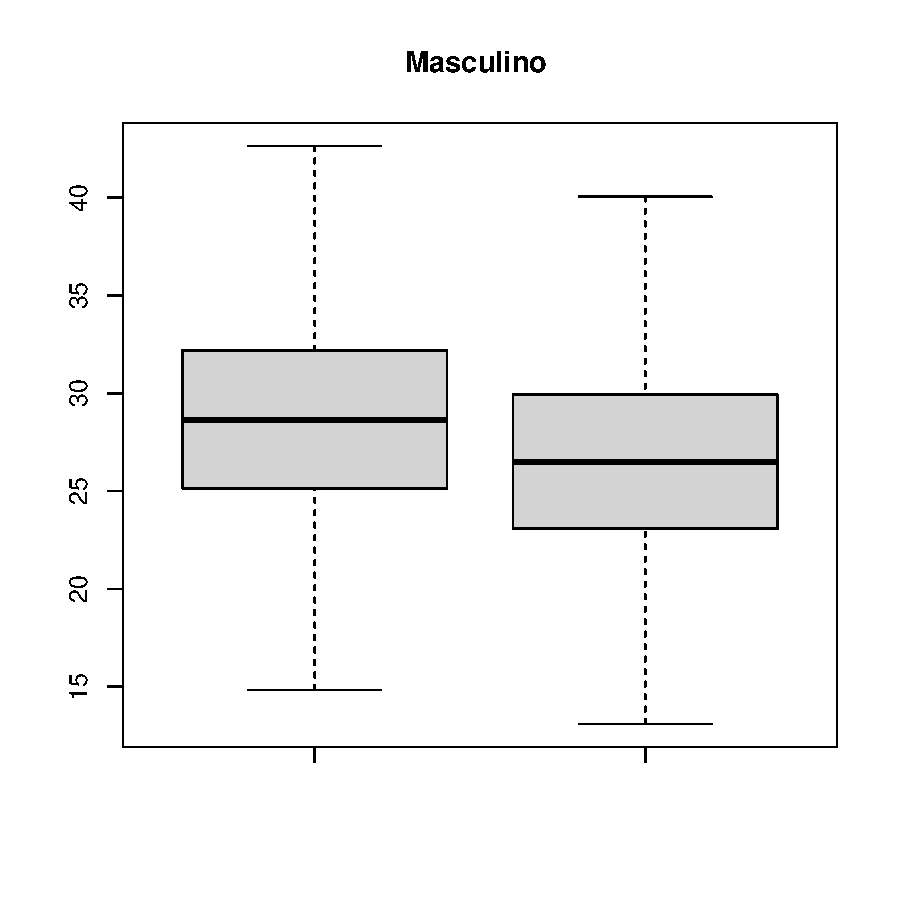
\includegraphics[width=.4\linewidth]{figure/minimal-boxplot-depois-1} 
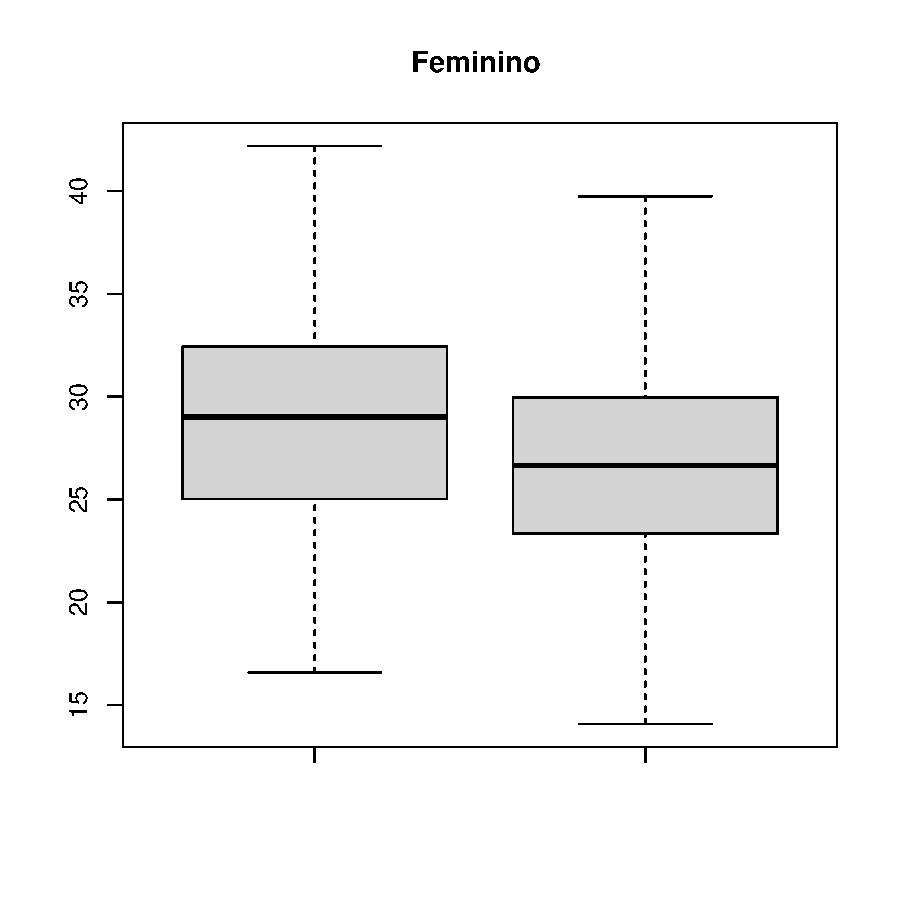
\includegraphics[width=.4\linewidth]{figure/minimal-boxplot-depois-2} 

}


\end{knitrout}
\caption{Diagrama de caixa de Y1 (un) e Y2 (un) (sexo masculino e feminino, respectivamente, UESC/BA - 2021.}
\end{figure}
\pagebreak

\subsection{Para Y1}

\textbf{1.2.1 (0.5)Apresentações tabulares }    
 %---------------------------masculina-----------------------------

% latex table generated in R 4.1.1 by xtable 1.8-4 package
% Tue Nov 09 12:59:06 2021
\begin{table}[!ht]
\centering
\caption{Tabela de distribuição de frequência de Y1 (sexo masculino), UESC/BA - 2021}
  \begin{tabular}{rlrrrrr} 
    \toprule
   & Class limits & f & rf & rf(\%) & cf & cf(\%) \\ 
    \midrule
  1 & [14.692,17.056) & 14.00 & 0.01 & 0.94 & 14.00 & 0.94 \\ 
    2 & [17.056,19.421) & 32.00 & 0.02 & 2.14 & 46.00 & 3.08 \\ 
    3 & [19.421,21.785) & 95.00 & 0.06 & 6.36 & 141.00 & 9.44 \\ 
    4 & [21.785,24.15) & 163.00 & 0.11 & 10.91 & 304.00 & 20.35 \\ 
    5 & [24.15,26.514) & 211.00 & 0.14 & 14.12 & 515.00 & 34.47 \\ 
    6 & [26.514,28.879) & 263.00 & 0.18 & 17.60 & 778.00 & 52.07 \\ 
    7 & [28.879,31.244) & 247.00 & 0.17 & 16.53 & 1025.00 & 68.61 \\ 
    8 & [31.244,33.608) & 206.00 & 0.14 & 13.79 & 1231.00 & 82.40 \\ 
    9 & [33.608,35.973) & 146.00 & 0.10 & 9.77 & 1377.00 & 92.17 \\ 
    10 & [35.973,38.337) & 85.00 & 0.06 & 5.69 & 1462.00 & 97.86 \\ 
    11 & [38.337,40.702) & 22.00 & 0.01 & 1.47 & 1484.00 & 99.33 \\ 
    12 & [40.702,43.066) & 10.00 & 0.01 & 0.67 & 1494.00 & 100.00 \\ 
     \bottomrule
  \end{tabular}
\end{table}

%---------------------------feminina----------------------------------

% latex table generated in R 4.1.1 by xtable 1.8-4 package
% Tue Nov 09 13:04:51 2021
\begin{table}[!ht]
\centering
\caption{Tabela de distribuição de frequência de Y1 (sexo feminino), UESC/BA - 2021}
  \begin{tabular}{rlrrrrr}
    \toprule
   & Class limits & f & rf & rf(\%) & cf & cf(\%) \\ 
    \midrule
  1 & [16.424,19.043) & 12.00 & 0.03 & 3.17 & 12.00 & 3.17 \\ 
    2 & [19.043,21.662) & 25.00 & 0.07 & 6.61 & 37.00 & 9.79 \\ 
    3 & [21.662,24.28) & 41.00 & 0.11 & 10.85 & 78.00 & 20.63 \\ 
    4 & [24.28,26.899) & 62.00 & 0.16 & 16.40 & 140.00 & 37.04 \\ 
    5 & [26.899,29.518) & 62.00 & 0.16 & 16.40 & 202.00 & 53.44 \\ 
    6 & [29.518,32.137) & 76.00 & 0.20 & 20.11 & 278.00 & 73.54 \\ 
    7 & [32.137,34.756) & 46.00 & 0.12 & 12.17 & 324.00 & 85.71 \\ 
    8 & [34.756,37.374) & 35.00 & 0.09 & 9.26 & 359.00 & 94.97 \\ 
    9 & [37.374,39.993) & 16.00 & 0.04 & 4.23 & 375.00 & 99.21 \\ 
    10 & [39.993,42.612) & 3.00 & 0.01 & 0.79 & 378.00 & 100.00 \\ 
     \bottomrule
  \end{tabular}
\end{table}
 \pagebreak
      \textbf{1.2.2 (0.5) Histograma e o polígono de freqüência acumulada}
\begin{figure}[!h]
\label{figura:Histograma-Poligono-M}
\begin{knitrout}
\definecolor{shadecolor}{rgb}{0.969, 0.969, 0.969}\color{fgcolor}

{\centering 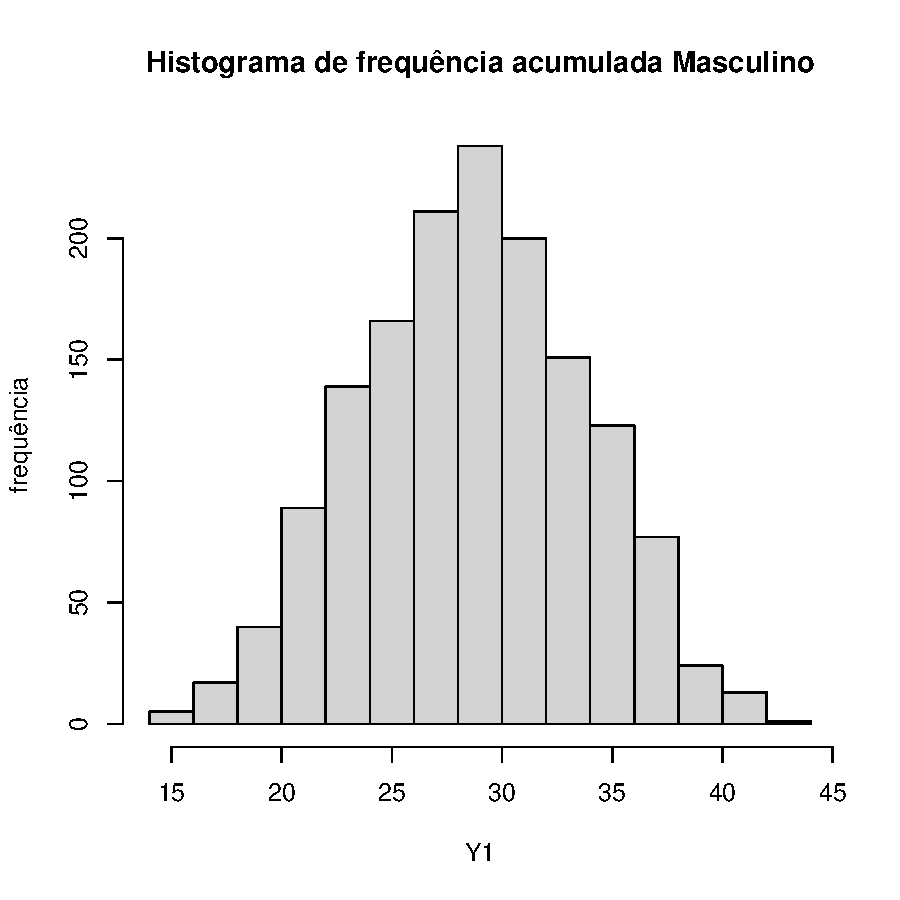
\includegraphics[width=.4\linewidth]{figure/minimal-Histograma-Poligono-Masc-1} 
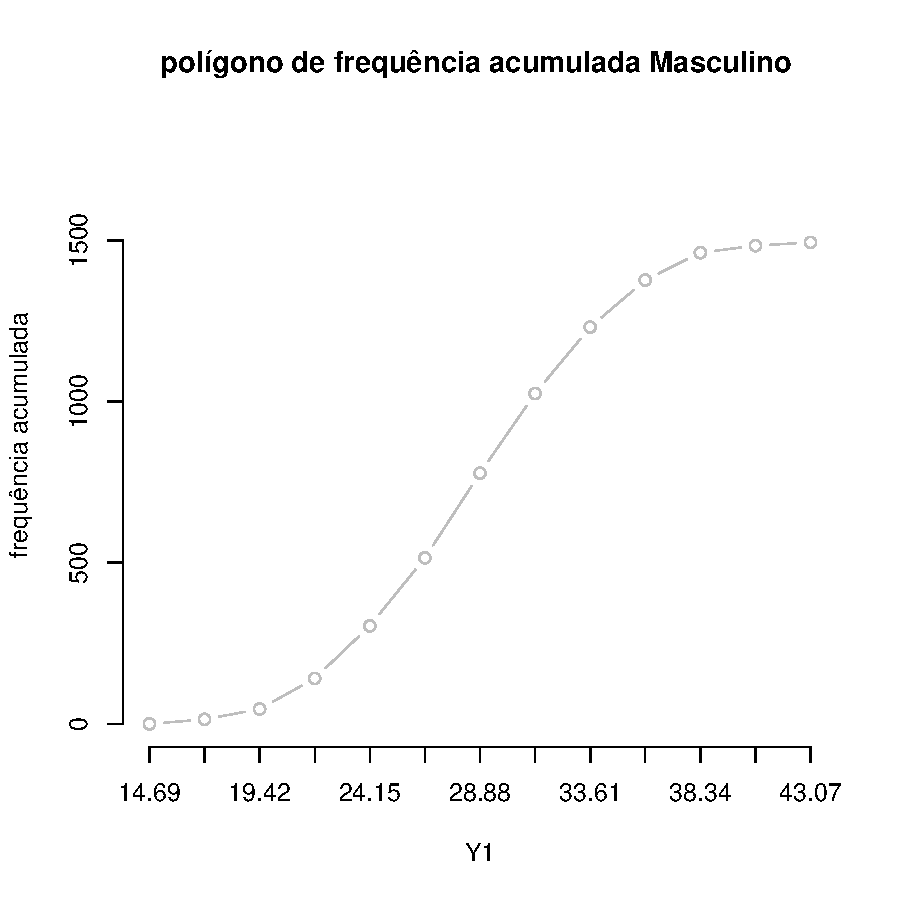
\includegraphics[width=.4\linewidth]{figure/minimal-Histograma-Poligono-Masc-2} 

}


\end{knitrout}
\caption{Histograma e polígono de frequência acumulada de Y1 (un) (sexo masculino), UESC/BA - 2021.
}
\end{figure}

\begin{figure}[!h]
\label{figura:Histograma-Poligono-F}
\begin{knitrout}
\definecolor{shadecolor}{rgb}{0.969, 0.969, 0.969}\color{fgcolor}

{\centering 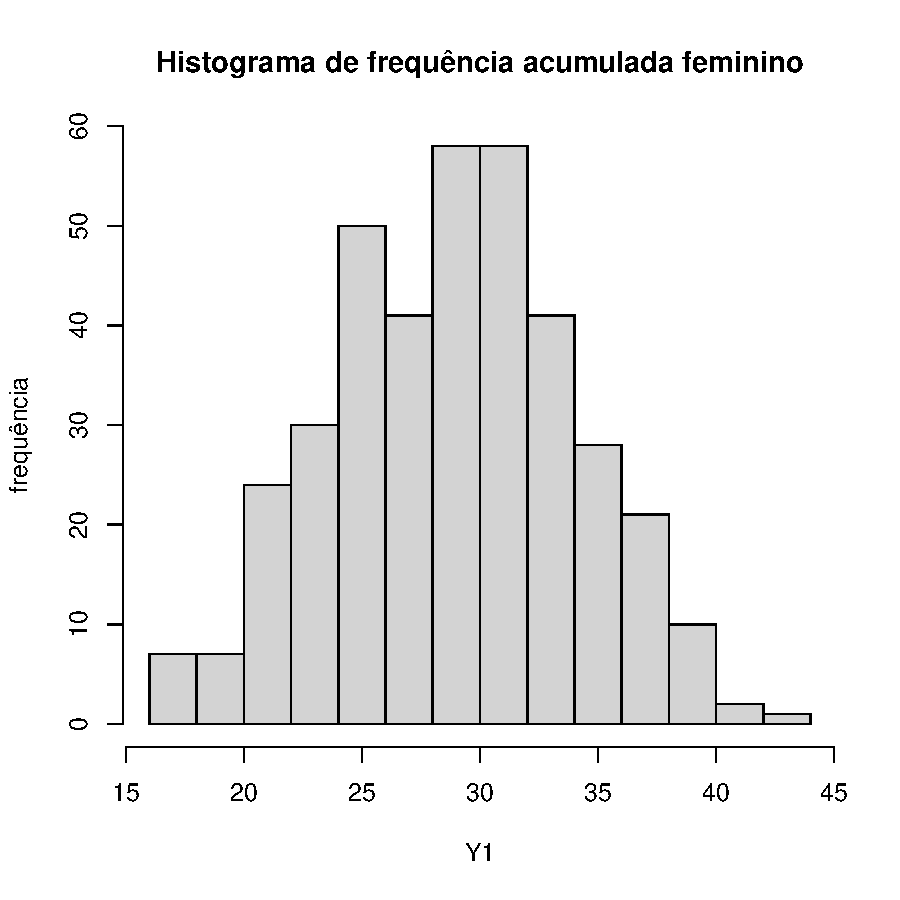
\includegraphics[width=.4\linewidth]{figure/minimal-Histograma-Poligono-Fem-1} 
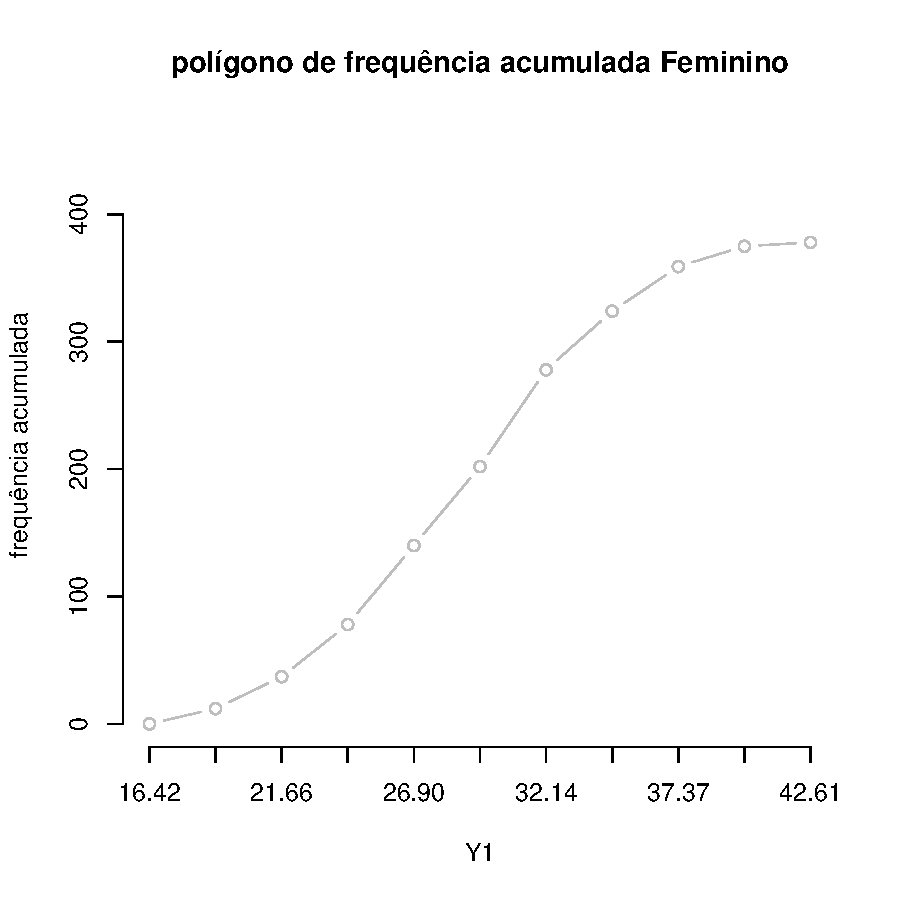
\includegraphics[width=.4\linewidth]{figure/minimal-Histograma-Poligono-Fem-2} 

}


\end{knitrout}
\caption{Histograma e polígono de frequência acumulada de Y1 (un) (sexo feminino), UESC/BA - 2021.
}
\end{figure}
\pagebreak

\section{AED: medidas estatísticas básicas(3.0).}

    \subsection{(1.5) AED: Medidas determinadas a partir dos vetores}
    
%-----------------------------------------------------------------------
    \textbf{ 2.1.1 (0.5) Tendência central}

 %---------------------------masculina-----------------------------

\begin{table}[!ht]
  \centering
  \caption{Medidas de tendêcia central (sexo masculino), UESC/BA - 2021}
  \begin{tabular}{rlrrr} 
    \toprule
    var & n & m & md \\ 
    \midrule
  Y1 & 28.66 & 27.81 & 28.63 \\ 
  Y2 & 26.43 & 31.01 & 26.49 \\ 
     \bottomrule
  \end{tabular}
\end{table}

%---------------------------feminina----------------------------------

\begin{table}[!ht]
  \centering
  \caption{Medidas de tendêcia central (sexo feminino), UESC/BA - 2021}
  \begin{tabular}{rlrrr}
    \toprule   
    var & n & m & md \\ 
    \midrule
  Y1 & 28.86 & 33.15 & 29.03 \\ 
  Y2 & 26.52 & 27.14 & 26.66 \\ 
     \bottomrule
  \end{tabular}
\end{table}
%-----------------------------------------------------------------------
\textbf{2.1.2 (0.5) Posição}

%----------------------------quartis-masculina----------------------------

\begin{table}[!ht]
  \centering
  \caption{Quartis dos usúarios (sexo masculino), UESC/BA - 2021}
\begin{tabular}{llll}
\hline
   & 25\%  & 50\%  & 75\%  \\ \hline
Y1 & 25.14 & 28.63 & 32.19 \\
Y2 & 23.09 & 26.49 & 29.93 \\ \hline
\end{tabular}
\end{table}
%---------------------------quartis-feminina------------------------------

\begin{table}[!ht]
  \centering
  \caption{Quartis dos usúarios (sexo feminino), UESC/BA - 2021}
\begin{tabular}{llll}
\hline
   & 25\%  & 50\%  & 75\%  \\ \hline
Y1 & 25.04 & 29.03 & 32.43 \\
Y2 & 23.36 & 26.66 & 29.99 \\ \hline
\end{tabular}
\end{table}
%--------------------------decis-masculina----------------------------

\begin{table}[!ht]
  \centering
  \caption{Decis dos usúarios (sexo Masculino), UESC/BA - 2021}
\begin{tabular}{llllllllll}
\hline
   & 10\%  & 20\%  & 30\%  & 40\%  & 50\%  & 60\%  & 70\%  & 80\%  & 90\%  \\ \hline
Y1 & 21.97 & 24.09 & 25.91 & 27.37 & 28.63 & 29.96 & 31.41 & 33.10 & 35.46 \\
Y2 & 20.00 & 22.10 & 23.77 & 25.26 & 26.49 & 27.71 & 29.12 & 30.79 & 32.64 \\ \hline
   &       &       &       &       &       &       &       &       &      
\end{tabular}
 \end{table}
%-----------------------decis-feminina-----------------------------------

\begin{table}[!ht]
  \centering
  \caption{Decis dos usúarios (sexo Feminino), UESC/BA - 2021}
  \begin{tabular}{rrr}
  \toprule
 & Y1 & Y2 \\ 
  \midrule
\begin{tabular}{llllllllll}
\hline
   & 10\%  & 20\%  & 30\%  & 40\%  & 50\%  & 60\%  & 70\%  & 80\%  & 90\%  \\ \hline
Y1 & 22.08 & 24.23 & 25.69 & 27.60 & 29.03 & 30.30 & 31.69 & 33.08 & 35.84 \\
Y2 & 19.27 & 22.51 & 24.06 & 25.49 & 26.66 & 28.02 & 29.21 & 31.11 & 35.27 \\ \hline
   &       &       &       &       &       &       &       &       &      
\end{tabular}
   \bottomrule
\end{tabular} 
\end{table}

\textbf{2.1.3 (0.5) Dispersão}



%---------------------------Dispersão_masculino---------------------------
\begin{table}[!ht]
  \centering
  \caption{Dispersão dos usuários (sexo masculino), UESC/BA - 2020}
 \begin{tabular}{rrrrr}
  \toprule
 & a.t & variância & d.padrão & c.v \\ 
  \midrule
1 & 27.80 & 25.56 & 5.06 & 17.64 \\ 
  2 & 26.96 & 23.34 & 4.83 & 18.27 \\ 
   \bottomrule
\end{tabular} 
\end{table}
       
%---------------------------Dispersão-feminino---------------------------
\begin{table}[!ht]
  \centering
  \caption{Dispersão dos usuários (sexo feminino), UESC/BA - 2020}
\begin{tabular}{rrrrr}
  \toprule
 & a.t & variância & d.padrão & c.v \\ 
  \midrule
1 & 25.60 & 26.79 & 5.18 & 17.94 \\ 
  2 & 25.66 & 25.53 & 5.05 & 19.05 \\ 
   \bottomrule
\end{tabular} 
\end{table}
%-----------------------------------------------------------------------------
\subsection{AED: Medidas determinadas a partir de apresentações tabulares (1.5)} 

 \begin{table}[!ht]
  \centering
  \caption{Tabela de distribuição de frequência recosntruída de publicação, UESC/BA - 2020}
   \begin{tabular}{rlrrr}
  \toprule
  \begin{tabular}{rlrrrrr}
  \toprule
 & Class limits & f & rf & rf($\backslash$\%) & cf & cf($\backslash$\%) \\ 
  \midrule
1 & [10,20) & 9.00 & 0.04 & 3.90 & 9.00 & 3.90 \\ 
  2 & [20,30) & 18.00 & 0.08 & 7.79 & 27.00 & 11.69 \\ 
  3 & [30,40) & 28.00 & 0.12 & 12.12 & 55.00 & 23.81 \\ 
  4 & [40,50) & 39.00 & 0.17 & 16.88 & 94.00 & 40.69 \\ 
  5 & [50,60) & 47.00 & 0.20 & 20.35 & 141.00 & 61.04 \\ 
  6 & [60,70) & 39.00 & 0.17 & 16.88 & 180.00 & 77.92 \\ 
  7 & [70,80) & 27.00 & 0.12 & 11.69 & 207.00 & 89.61 \\ 
  8 & [80,90) & 17.00 & 0.07 & 7.36 & 224.00 & 96.97 \\ 
  9 & [90,100) & 7.00 & 0.03 & 3.03 & 231.00 & 100.00 \\ 
   \bottomrule
\end{tabular}
  \end{table}

\subsection{(0.5) Tendência central}

\begin{table}[!ht]
  \centering
  \caption{Medidas de tendêcia central, UESC/BA - 2021}
  \begin{tabular}{rlrrr}
  \toprule
 & var & n & m & md \\ 
  \midrule
 medidas & 54.44 & 55.00 & 54.57 \\ 
   \bottomrule
\end{tabular}
\end{table}

\textbf{2.1.2 (0.5) Posição}


\begin{table}[!ht]
  \centering
  \caption{Quartis dos usúarios, UESC/BA - 2021}
  \centering
  \begin{tabular}{rrrr}
  \hline
   & 10\% & 20\% & 30\% \\ 
  \hline
  medidas & 40.71 & 54.57 & 68.27 \\ 
   \hline
\end{tabular}
\end{table}

\begin{table}[!ht]
  \centering
  \caption{Decis dos usúarios, UESC/BA - 2021}
  \begin{tabular}{rrrrrrrrrr}
  \hline
 & 10\% & 20\% & 30\% & 40\% & 50\% & 60\% & 70\% & 80\% & 90\% \\ 
  \hline
medidas & 27.83 & 36.86 & 43.67 & 49.59 & 54.57 & 59.49 & 65.31 & 71.78 & 80.53 \\ 
   \hline
\end{tabular}
\end{table}

\subsection{(0.5) Dispersão}

%---------------------------Dispersão---------------------------
\begin{table}[!ht]
    \centering
    \caption{Dispersão dos usuários, UESC/BA - 2020}
    \centering
  \begin{tabular}{rrrr}
    \hline
   & variância & d.padrão & c.v \\ 
    \hline
  1 & 377.51 & 19.43 & 2.80 \\
     \hline
  \end{tabular}
\end{table}
 
 \section{AED: Medidas estatísticas de associação e regressão linear (4.0)}
 \subsection{(1.5) Associação}

%---------------------covariância e correlação linerar simples-------------------                                                                 
  \textbf{3.1.1 (0.5) Estimativas: covariância e correlação linerar simples }
  

\begin{table}[!ht]
    \centering
    \caption{Matriz de variâncias e covariâncias (sexo masculino), UESC/BA - 2021}
    \begin{tabular}{rrr}
    \hline
    & Y1 & Y2 \\ 
    \hline
    Y1 & 25.56 & 23.00 \\ 
    Y2 & 23.00 & 23.34 \\ 
     \hline
  \end{tabular}
\end{table}

\begin{table}[!ht]
   \centering
   \caption{Matriz de variâncias e covariâncias (sexo feminino), UESC/BA - 2021}
   \begin{tabular}{rrr}
   \hline
  & Y1 & Y2\\ 
  \hline
  Y1 & 26.79 & -20.63 \\ 
  Y2 & -20.63 & 25.53 \\ 
   \hline
\end{tabular}
\end{table}

\begin{table}[!ht]
   \centering
   \caption{Matriz de correlações lineares simples (sexo masculino), UESC/BA - 2021}
   \begin{tabular}{rrr}
   \hline
  & Y1 & Y2\\ 
  \hline
  Y1 & 1.00 & -0.79 \\ 
  Y2 & -0.79 & 1.00 \\
  \hline
  \end{tabular}
\end{table}

\begin{table}[!ht]
  \centering
  \caption{Matriz de correlações lineares simples (sexo feminino), UESC/BA - 2021}
  \begin{tabular}{rrr}
   \hline
  & Y1 & Y2\\ 
  \hline
  Y1 & 1.00 & -0.79 \\ 
  Y2 & -0.79 & 1.00 \\ 
  \hline
  \end{tabular}
\end{table}
%---------------------------diagrama_dispersão---------------------------
  \textbf{3.1.2 (0.5) Diagrama de dispersão dos dados}
\begin{figure}[!h]
\label{figura:Diagrama de dispersão}
\begin{knitrout}
\definecolor{shadecolor}{rgb}{0.969, 0.969, 0.969}\color{fgcolor}

{\centering \includegraphics[width=.4\linewidth]{figure/minimal-Diagrama_de_dispersão_dos_Dados-1} 
\includegraphics[width=.4\linewidth]{figure/minimal-Diagrama_de_dispersão_dos_Dados-2} 

}


\end{knitrout}
\caption{Diagrama de dispersão de Y1 (un) e Y2 (un) (sexo masculino e feminino, respectivamente), UESC/BA - 2021.}
\end{figure}

  
  \textbf{3.1.3 (0.5) Comparação de estudos semelhantes}

\subsection{3.2 Regressão linear (2.5)}

  \textbf{3.2.1 (1.0) Ajustamento}


\begin{table}[!ht]
\centering
\caption{Polinômio grau I, UESC/BA - 2021}
\begin{tabular}{rrrrr}
  \hline
 & Estimate & Std. Error & t value & Pr($>$$|$t$|$) \\ 
  \hline
(Intercept) & 1.7291 & 0.6237 & 2.77 & 0.0242 \\ 
  x & 1.3072 & 0.1052 & 12.43 & 0.0000 \\ 
   \hline
\end{tabular}
\end{table}

\begin{table}[!ht]
\centering
\caption{Polinômio grau II, UESC/BA - 2021}
\begin{tabular}{rrrrr}
  \hline
 & Estimate & Std. Error & t value & Pr($>$$|$t$|$) \\ 
  \hline
(Intercept) & 0.6429 & 0.6431 & 1.00 & 0.3508 \\ 
  x & 2.0405 & 0.2995 & 6.81 & 0.0003 \\ 
  I(x\verb|^|2) & -0.0733 & 0.0288 & -2.54 & 0.0385 \\ 
   \hline 
   \hline
\end{tabular}
\end{table}

  \textbf{3.2.2 (0.5) Diagrama de dispersão com modelos ajustados}
  
\begin{figure}[!h]
\label{figura:Diagrama de dispersão_ajustado}
\begin{knitrout}
\definecolor{shadecolor}{rgb}{0.969, 0.969, 0.969}\color{fgcolor}\begin{kframe}
\begin{verbatim}
## integer(0)
## integer(0)
\end{verbatim}
\end{kframe}

{\centering \includegraphics[width=.4\linewidth]{figure/minimal-Diagrama_de_dispersão_ajustado-1} 
\includegraphics[width=.4\linewidth]{figure/minimal-Diagrama_de_dispersão_ajustado-2} 

}


\end{knitrout}
\caption{Diagrama de dispersão dos dados, modelos ajustados e respectivos r², UESC/BA - 2021.}
\end{figure}
  \textbf{3.2.3 (0.5) Qual modelo melhor explica o fenômeno em estudo?}
  
  \textbf{3.2.4 (0.5) Critérios de ajustamento e escolha de modelos}
           
\subsection{ Contextualização (1.0))}
\end{document}
